\documentclass[a4paper,12pt]{ujarticle}
\usepackage{listings,jlisting}
\usepackage[dvips]{graphicx}
\usepackage{siunitx}
\begin{document}
\title{マイクロコンピュータ}
\author{E1533 西総一朗}
\maketitle
\clearpage
\tableofcontents
\clearpage
\section{リスト5.1(LED点灯プログラム1)}
  \subsection{フローチャート}
  \begin{figure}[htbp]
   \begin{center}
    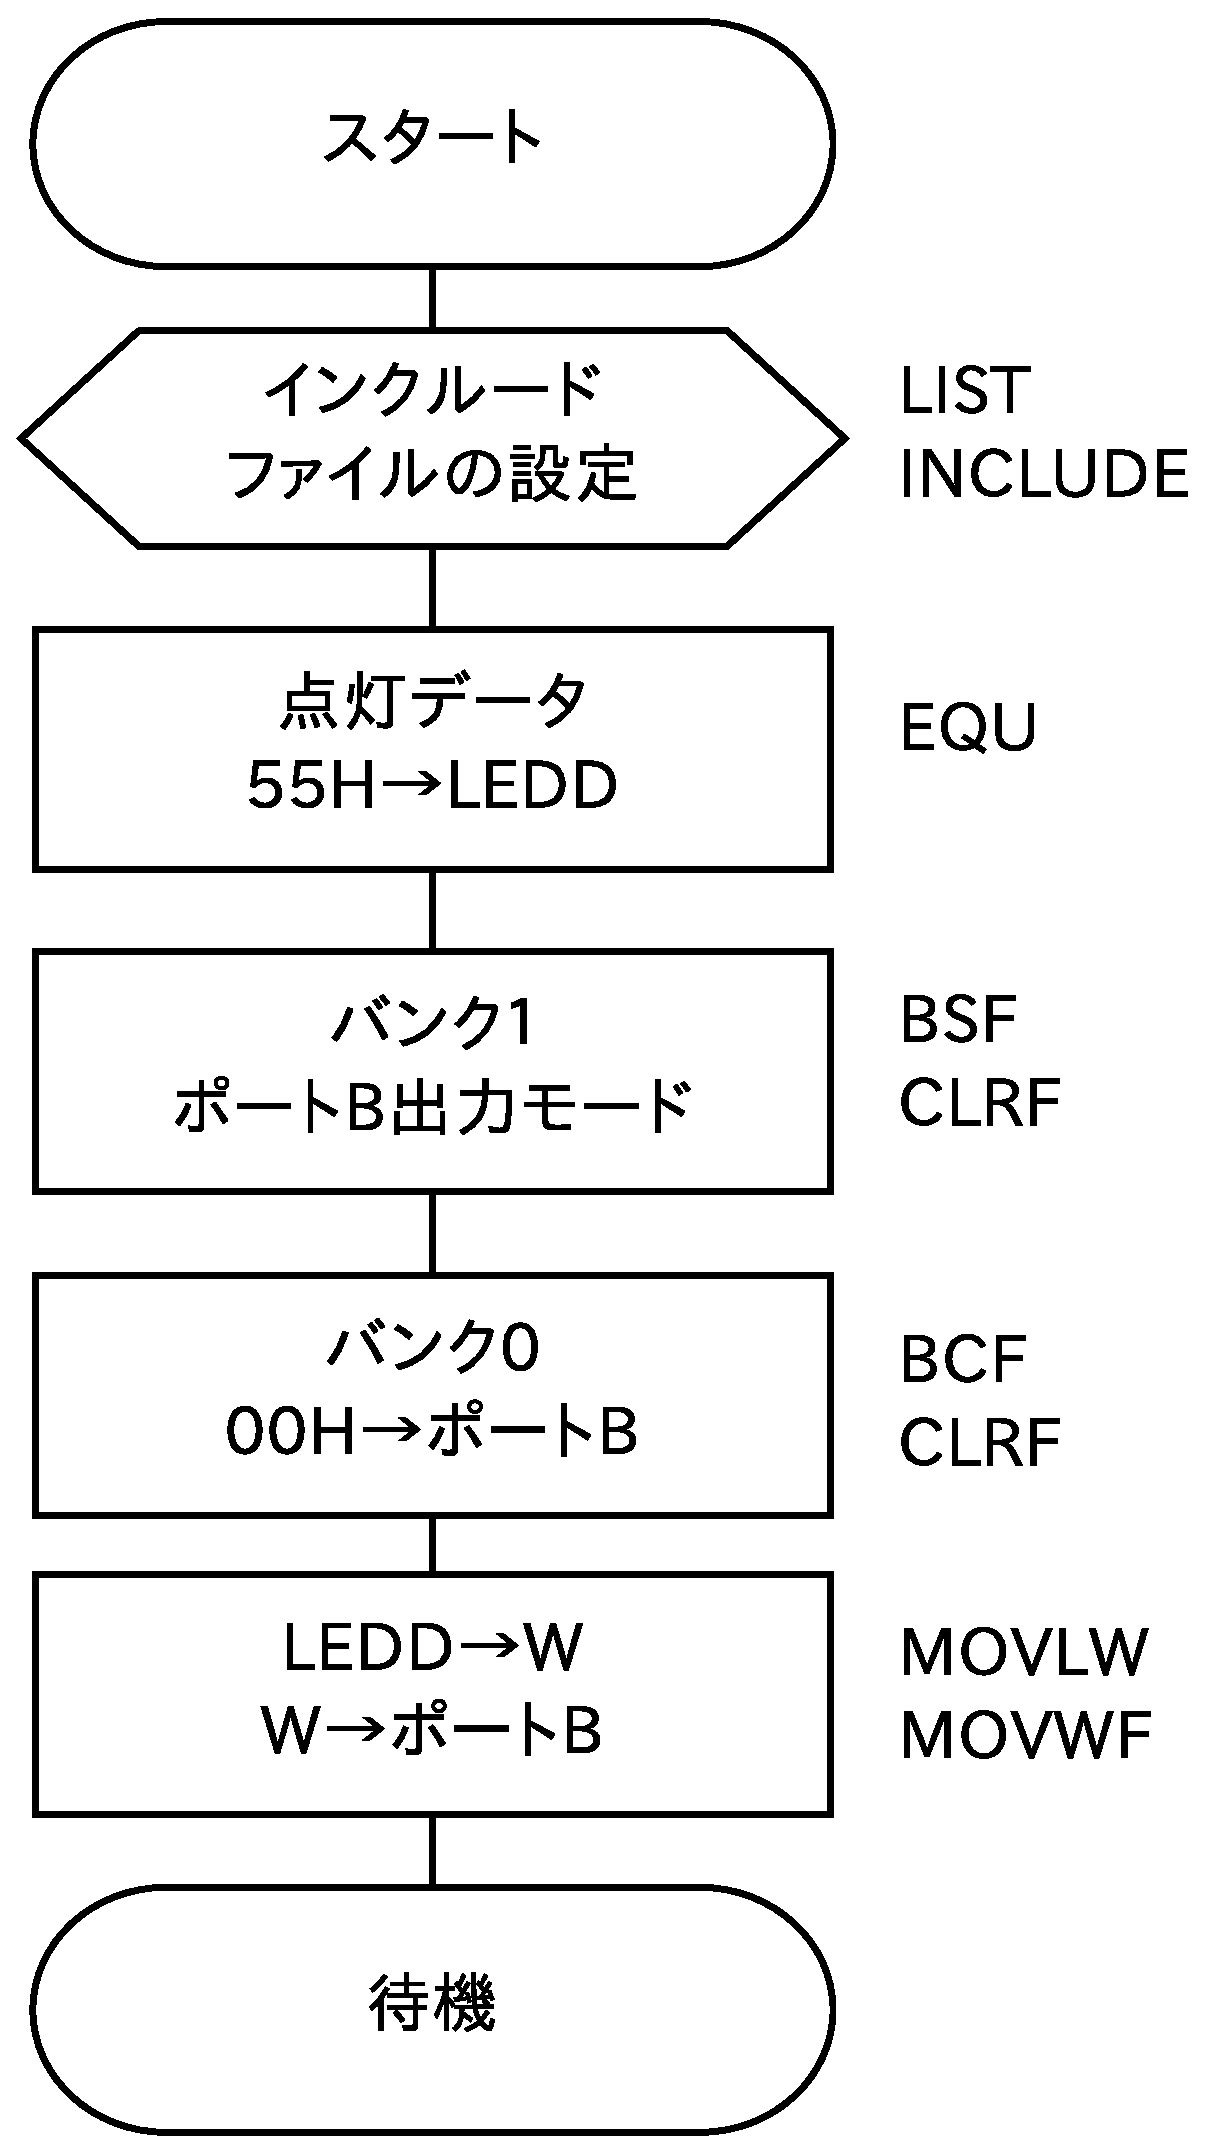
\includegraphics[height=140mm]{Diagram5-1.eps}
   \end{center}
   \caption{フローチャート}
   \label{fig}
  \end{figure}
  \clearpage
  \subsection{ソースコード}
  \begin{lstinputlisting}[basicstyle=\ttfamily\footnotesize, frame=single]
   {../5-1/5-1.asm}
  \end{lstinputlisting}
  \subsection{実行結果}
  \begin{eqnarray*}
   ○●○●○●○● \\
   ●:点灯○:消灯
  \end{eqnarray*}
  のようにLEDが点灯した。
  \subsection{考察}
  LEDDで宣言している16進数の点灯データを2進数に変換した
  \[
  55_{16} = 01010101_2
  \]
  の1のところが点灯したと考えられる。

  \subsection{練習問題5.1}
  例えば、
   \begin{eqnarray*}
    ○○●●●○○○ \\
    ●:点灯○:消灯
   \end{eqnarray*}
   のように点灯させたければ
   \[
    00111000_2 = 38_{16}
   \]
   なので、点灯データを38Hとすれば良い。
 \clearpage
 \section{リスト5-2(タイマの基本プログラム)}
  \subsection{フローチャート}
   \begin{figure}[htbp]
    \begin{center}
     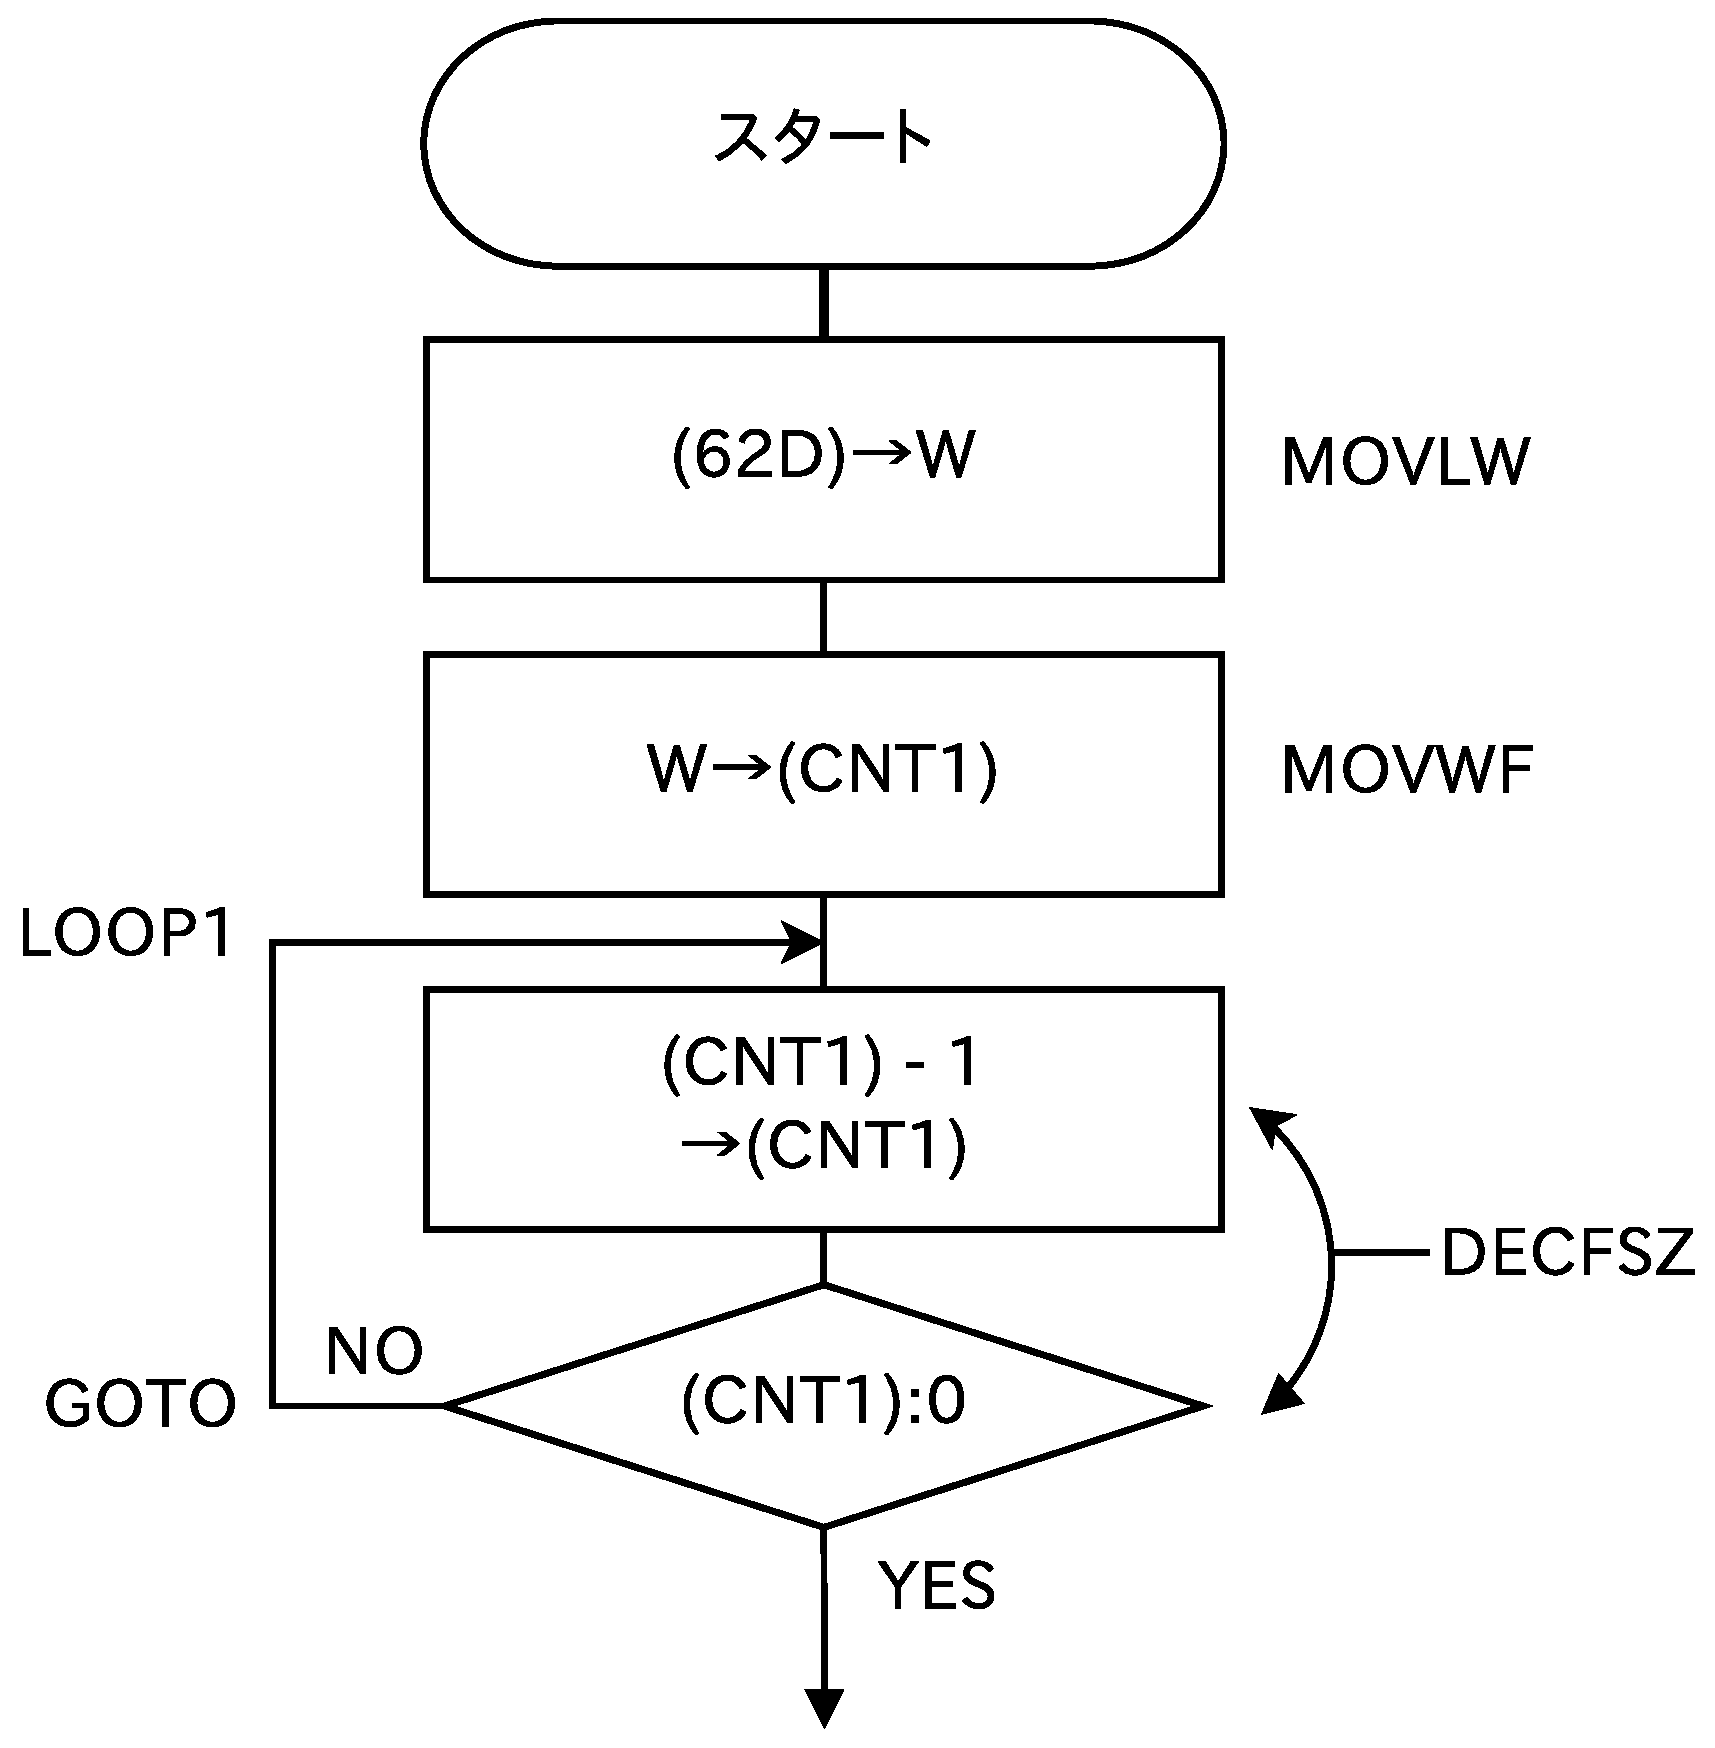
\includegraphics[height=100mm]{Diagram5-2.eps}
    \end{center}
    \caption{フローチャート}
    \label{fig}
   \end{figure}
  \subsection{ソースコード}
    \begin{lstinputlisting}[basicstyle=\ttfamily\footnotesize, frame=single]
     {../5-2/5-2.asm}
    \end{lstinputlisting}
    \subsection{考察}
    PICのクロック周波数は$10\si{\mega\hertz}$なので、1クロックあたりは
    \[
     \frac{1}{10\si{\mega\hertz}} = \SI{0.1}{\mu\second}
    \]
    4クロックで1サイクルなので、1サイクルあたりは
    \[
     \SI{0.1}{\mu\second} \times 4 = \SI{0.4}{\mu\second}
    \]
    \begin{figure}[htbp]
     \begin{center}
      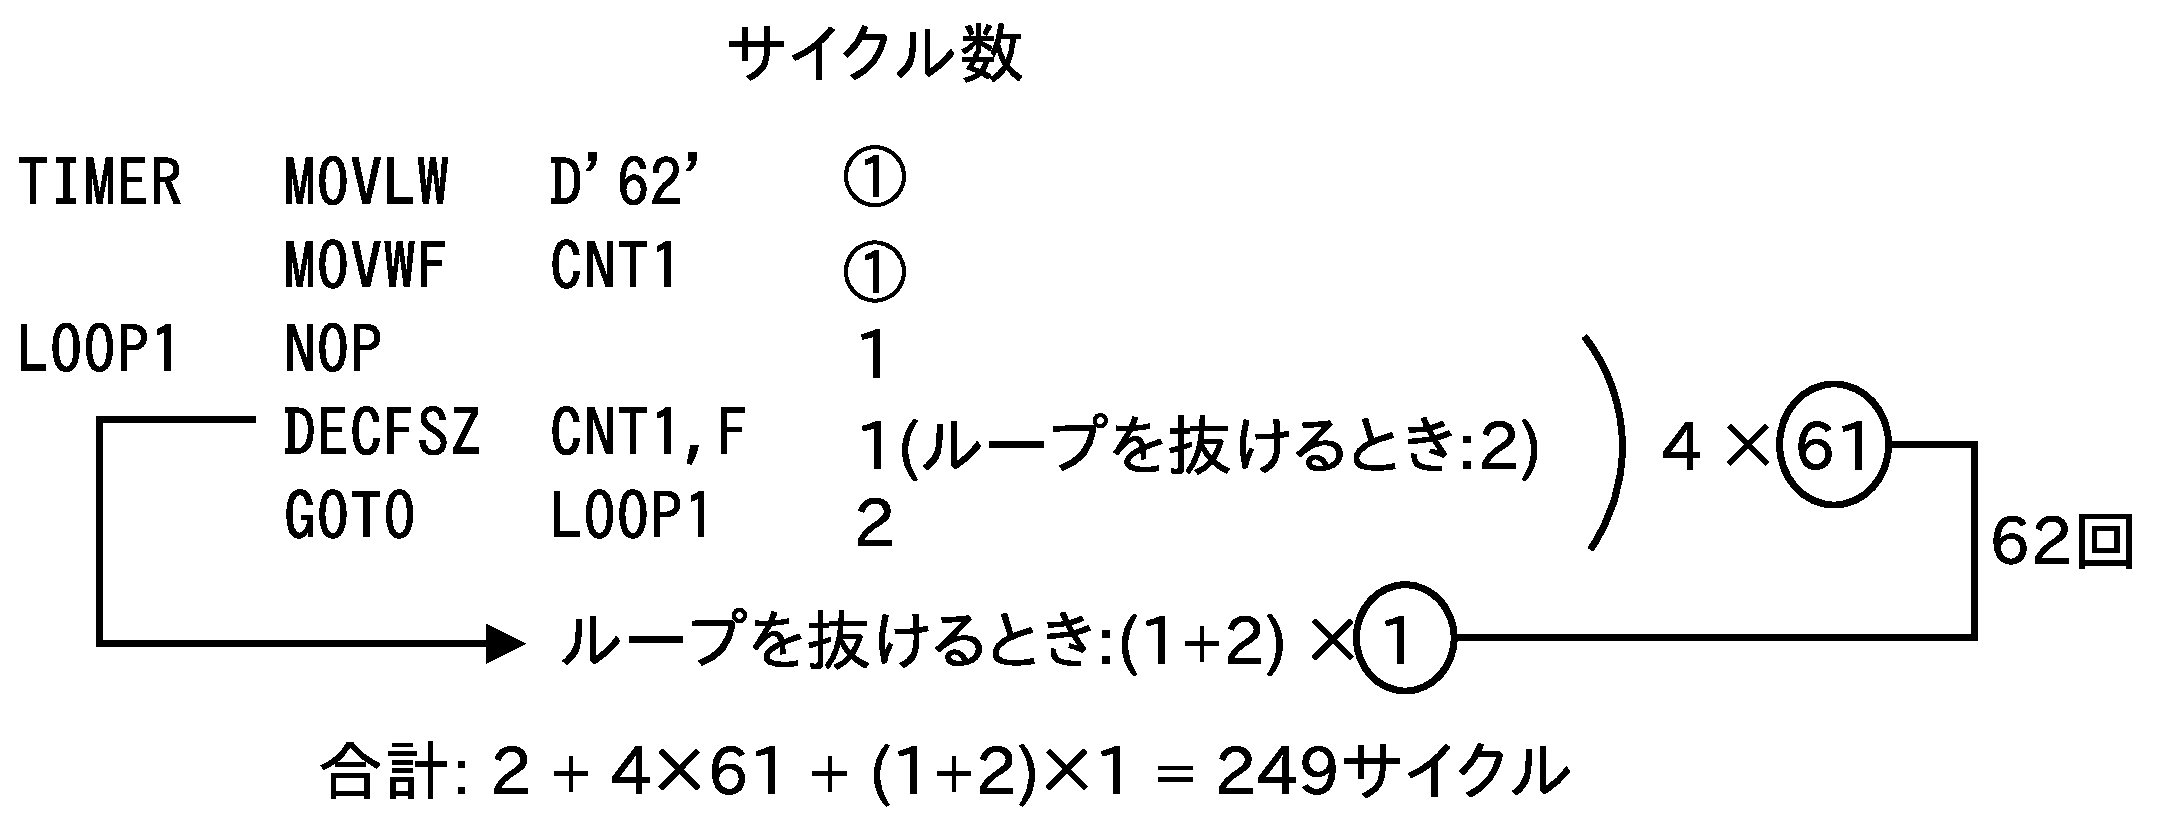
\includegraphics[width=130mm]{Diagram5-2-1.eps}
     \end{center}
     \caption{サイクル数}
     \label{fig}
    \end{figure}

    このループのサイクル数は$249$サイクルなので、
    \[
     \SI{0.4}{\mu\second} \times 249 = \SI{99.6}{\mu\second} =  \SI{0.1}{\milli\second}
    \]
    となり、このループでは$\SI{0.1}{\milli\second}$が消費される。
    \clearpage
 \section{リスト5-3(10秒タイマプログラム)}
 \subsection{フローチャート}
 \begin{figure}[htbp]
    \begin{center}
     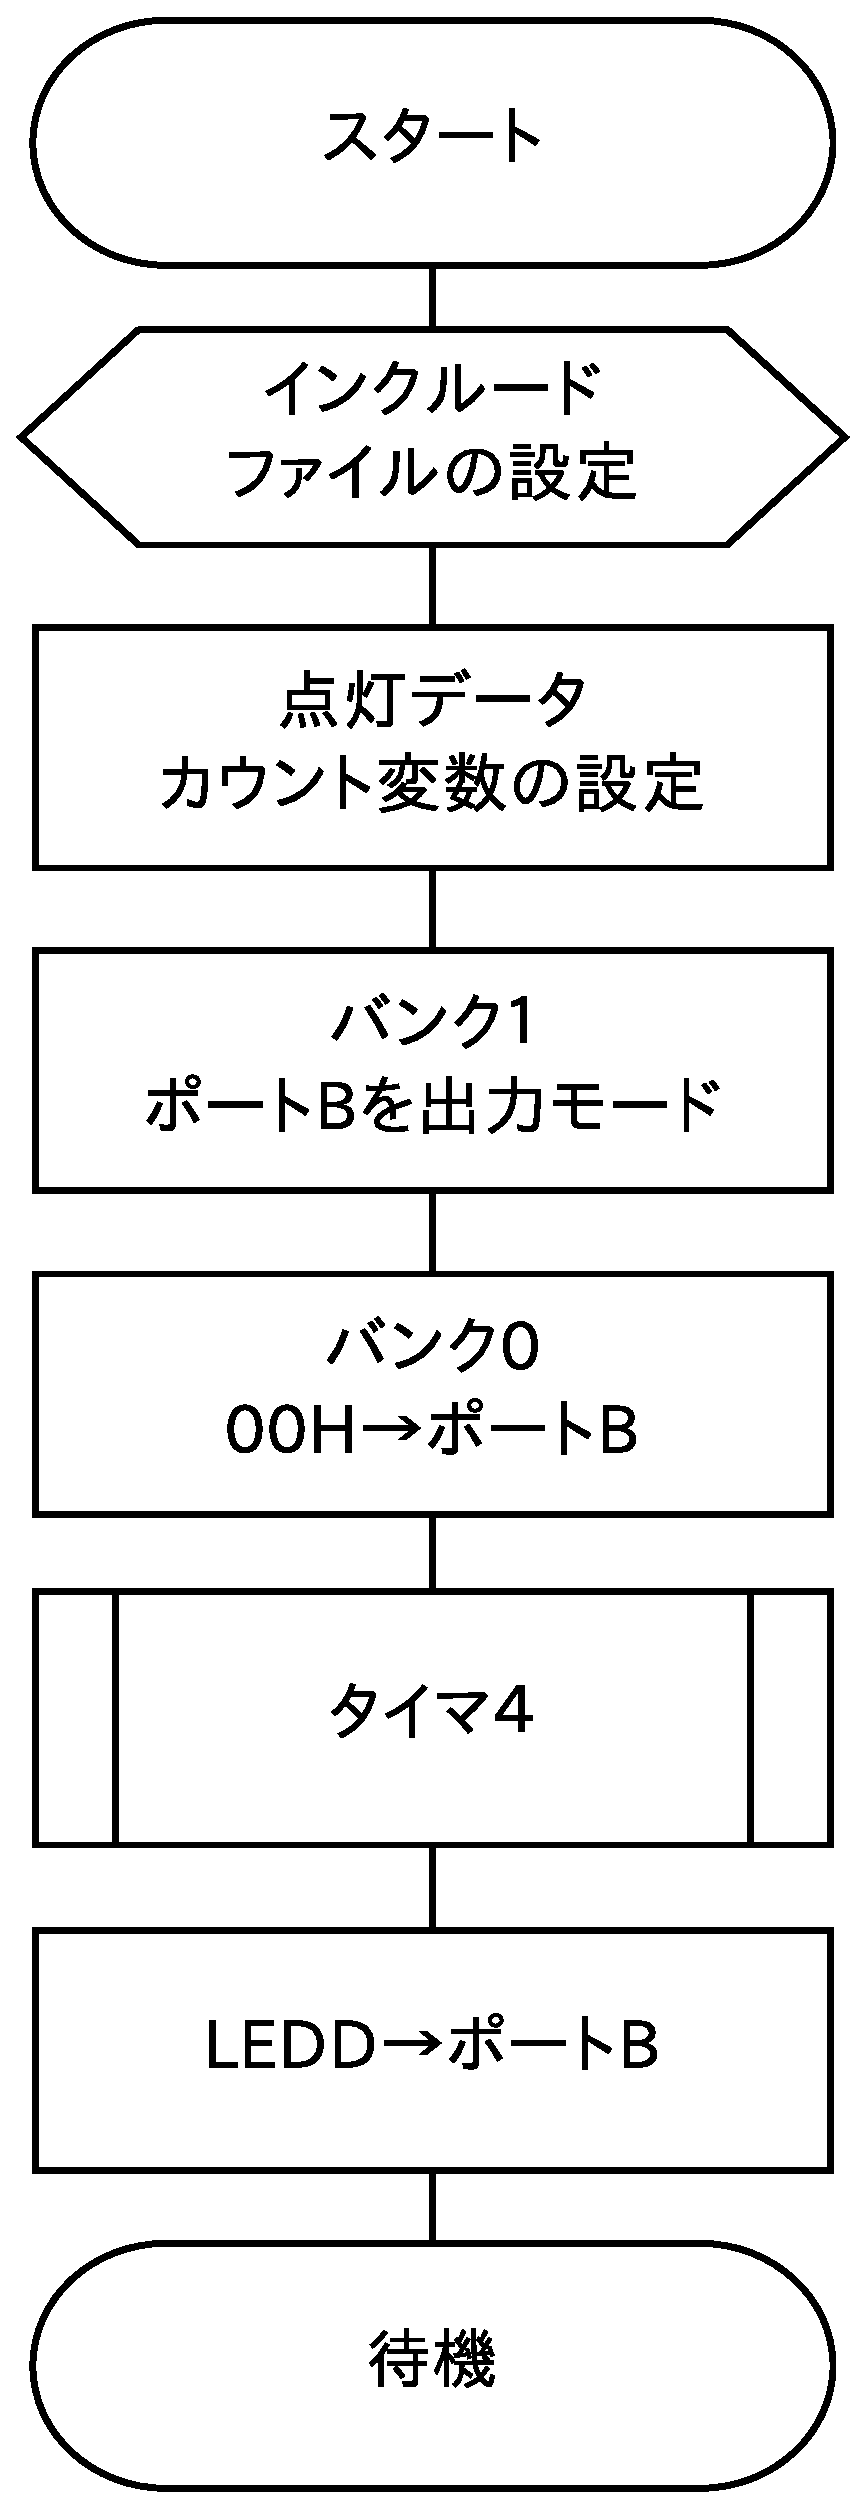
\includegraphics[height=145mm]{Diagram5-3.eps}
    \end{center}
    \caption{フローチャート}
    \label{fig}
 \end{figure}
 \clearpage
 \subsection{ソースコード}
  \begin{lstinputlisting}[basicstyle=\ttfamily\footnotesize, frame=single]
   {../5-3/5-3.asm}
  \end{lstinputlisting}
  \subsection{実行結果}
  10秒後に
  \begin{eqnarray*}
   {FF}_{16} = 11111111_2 \\
   ●●●●●●●● \\
   ●:点灯○:消灯
  \end{eqnarray*}
  こののようにすべてのLEDが点灯する。
  \subsection{考察}
  \[
    \SI{0.1}{\milli\second}\{timer1\} \times 100\{timer2\} \times 100\{timer3\} \times 10\{timer4\} = \SI{10}{\second}
  \]
  リスト5-2の\SI{0.1}{\milli\second}タイマのサブルーチンを100000回呼び出こすことで、10秒タイマを実装してる。
  \subsection{練習問題5.2}
  リスト5-2の\SI{0.1}{\milli\second}タイマのサブルーチンを5000回呼び出すことで、0.5秒タイマにする
   \begin{lstinputlisting}[basicstyle=\ttfamily\footnotesize, frame=single]
   {../5-3/5-3-1.asm}
   \end{lstinputlisting}
   \subsection{練習問題5.3}
   クロック周波数が$\SI{4}{\mega\hertz}$なので、1クロックあたりは
   \[
     \frac{1}{4\si{\mega\hertz}} = \SI{0.25}{\mu\second}
   \]
   4クロックで1サイクルなので、1サイクルあたりは
   \[
     \SI{0.25}{\mu\second} \times 4 = \SI{1}{\mu\second}
   \]
   つまり1サイクルで目的の$\SI{1}{\mu\second}$のタイマになるので、
   \begin{lstinputlisting}[basicstyle=\ttfamily\footnotesize, frame=single]
    {../5-3/5-3-2.asm}
   \end{lstinputlisting}
   となる。
   \clearpage
 \section{リスト5-4(LED点滅プログラム)}
   \subsection{フローチャート}
   \begin{figure}[htbp]
    \begin{center}
     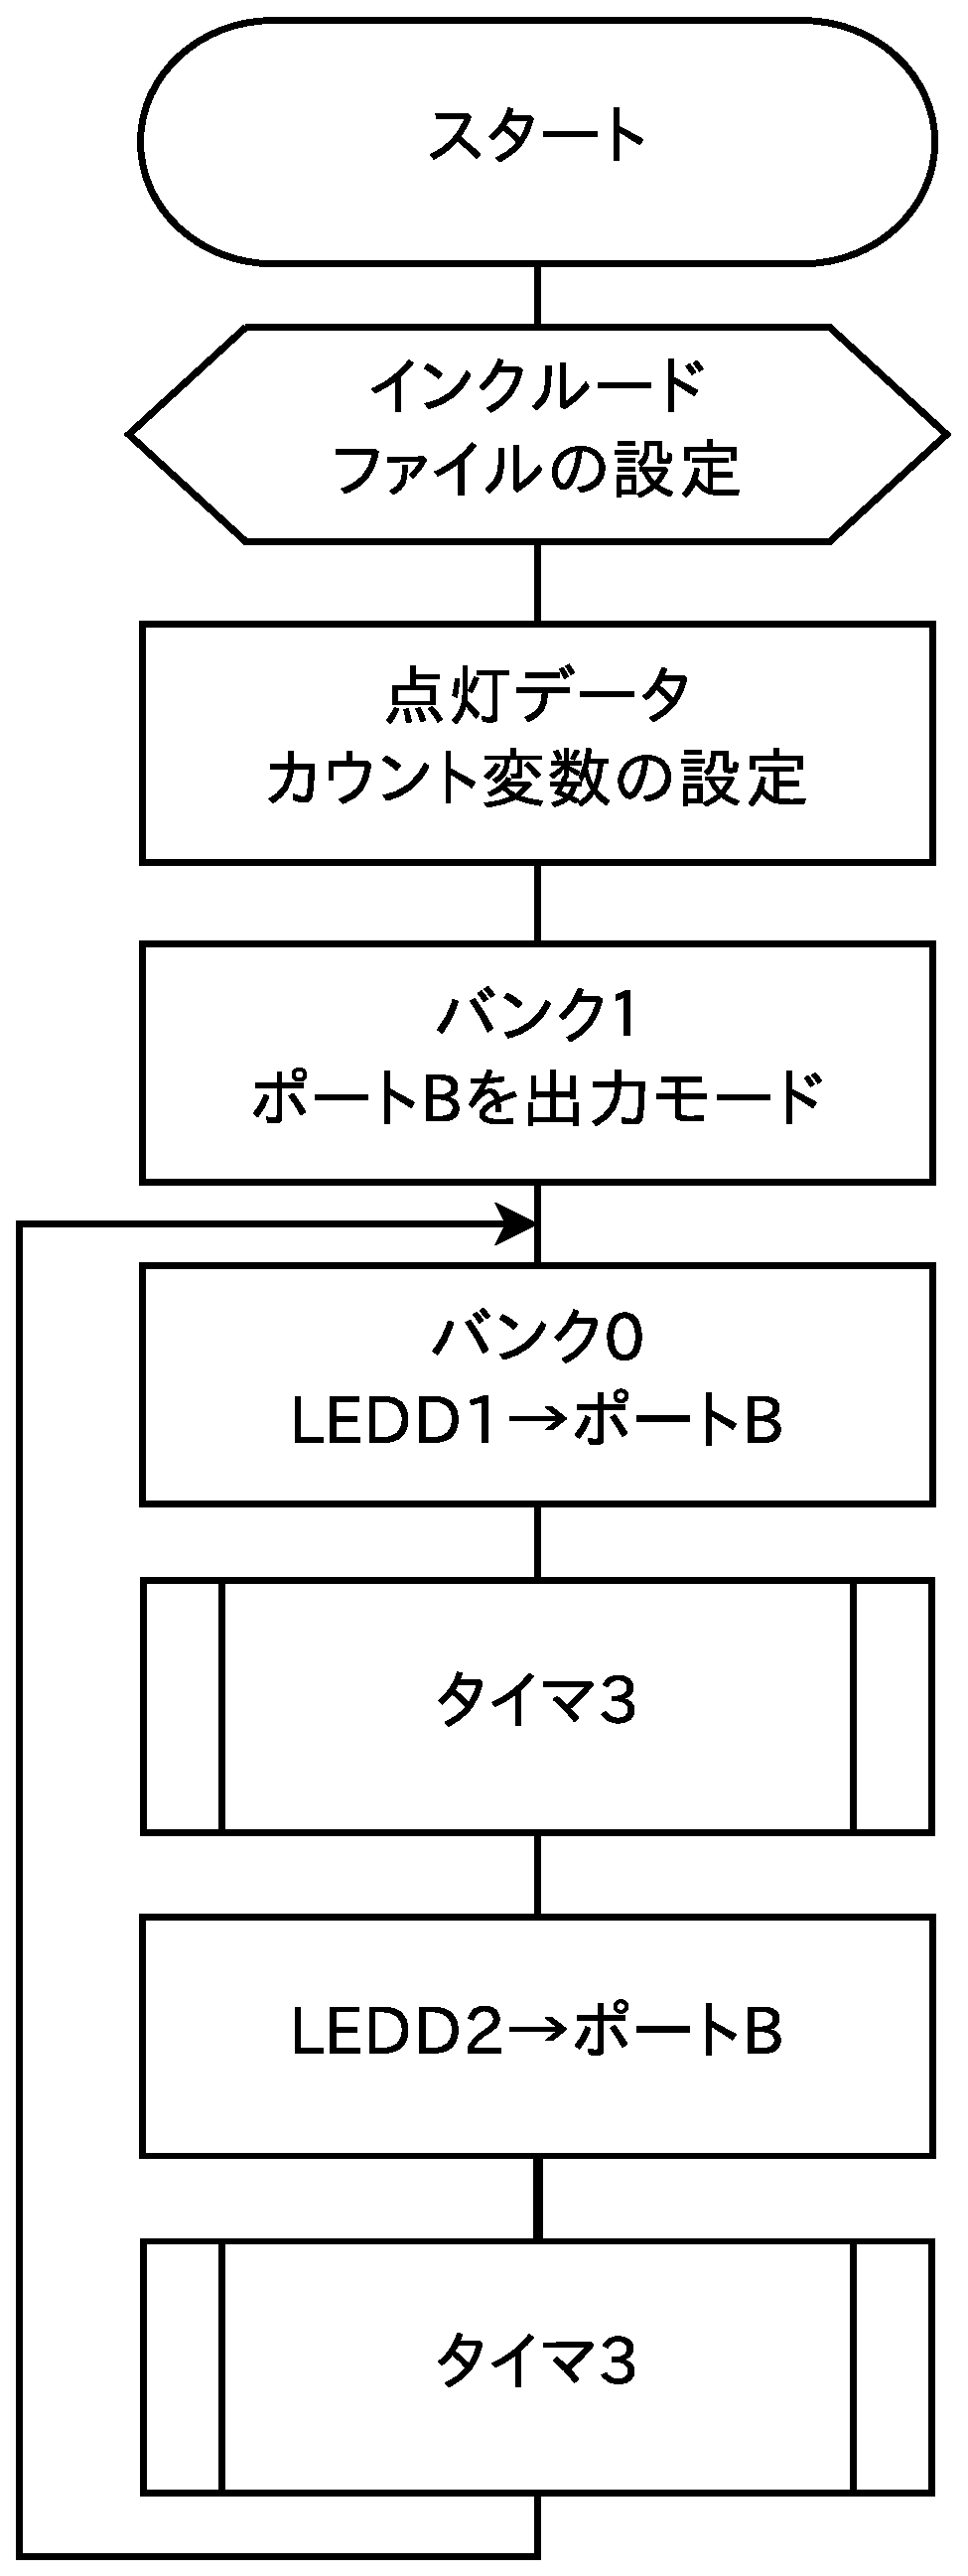
\includegraphics[height=145mm]{Diagram5-4.eps}
    \end{center}
    \caption{フローチャート}
    \label{fig}
   \end{figure}
   \clearpage
   \subsection{ソースコード}
   \begin{lstinputlisting}[basicstyle=\ttfamily\footnotesize, frame=single]
    {../5-4/5-4.asm}
   \end{lstinputlisting}
   \subsection{実行結果}
   \begin{eqnarray*}
    {AA}_{16} = 10101010_2 \\
    ●○●○●○●○ \\
    \\
    {55}_{16} = 01010101_2 \\
    ○●○●○●○● \\
    ●:点灯○:消灯
   \end{eqnarray*}
   この2つを1秒ごとに繰り返す。
   \subsection{考察}
    \[
    \SI{0.1}{\milli\second}\{timer1\} \times 100\{timer2\} \times 100\{timer3\}  = \SI{1}{\second}
    \]
    リスト5-2の\SI{0.1}{\milli\second}タイマのサブルーチンを1000回呼び出こすことで、1秒タイマを実装してる。
    \clearpage
  \subsection{練習問題5.4}
  例えば、
  \begin{eqnarray*}
    ●●○○○●●● \\
    \\
    ○○●●●○○○ \\
    ●:点灯○:消灯
  \end{eqnarray*}
  のように点灯させたければ、
  \begin{lstlisting}[basicstyle=\ttfamily\footnotesize, frame=single]
LEDD1   EQU     C7H
LEDD2   EQU     38H
  \end{lstlisting}
  のように点灯データをセットしてやればいい。
  \subsection{練習問題5.5}
  点滅の間隔を2秒にするには、
  \begin{lstlisting}[basicstyle=\ttfamily\footnotesize, frame=single]
TIMER1  MOVLW   D'62'       ;0.1ms
        MOVWF   CNT1
LOOP1   NOP
        DECFS Z CNT1,F
        GOTO    LOOP1
        RETURN

TIMER2  MOVLW   D'100'      ;10ms
        MOVWF   CNT2
LOOP2   NOP
        CALL    TIMER1
        DECFSZ  CNT2,F
        GOTO    LOOP2
        RETURN

TIMER3  MOVLW   D'200'      ;2s
        MOVWF   CNT3
LOOP3   NOP
        CALL    TIMER2
        DECFSZ  CNT3,F
        GOTO    LOOP3
  \end{lstlisting}
  このようにする。
 \section{リスト5-5(光が流れるプログラム(片道バージョン))}
  \subsection{フローチャート}
  \begin{figure}[htbp]
    \begin{center}
     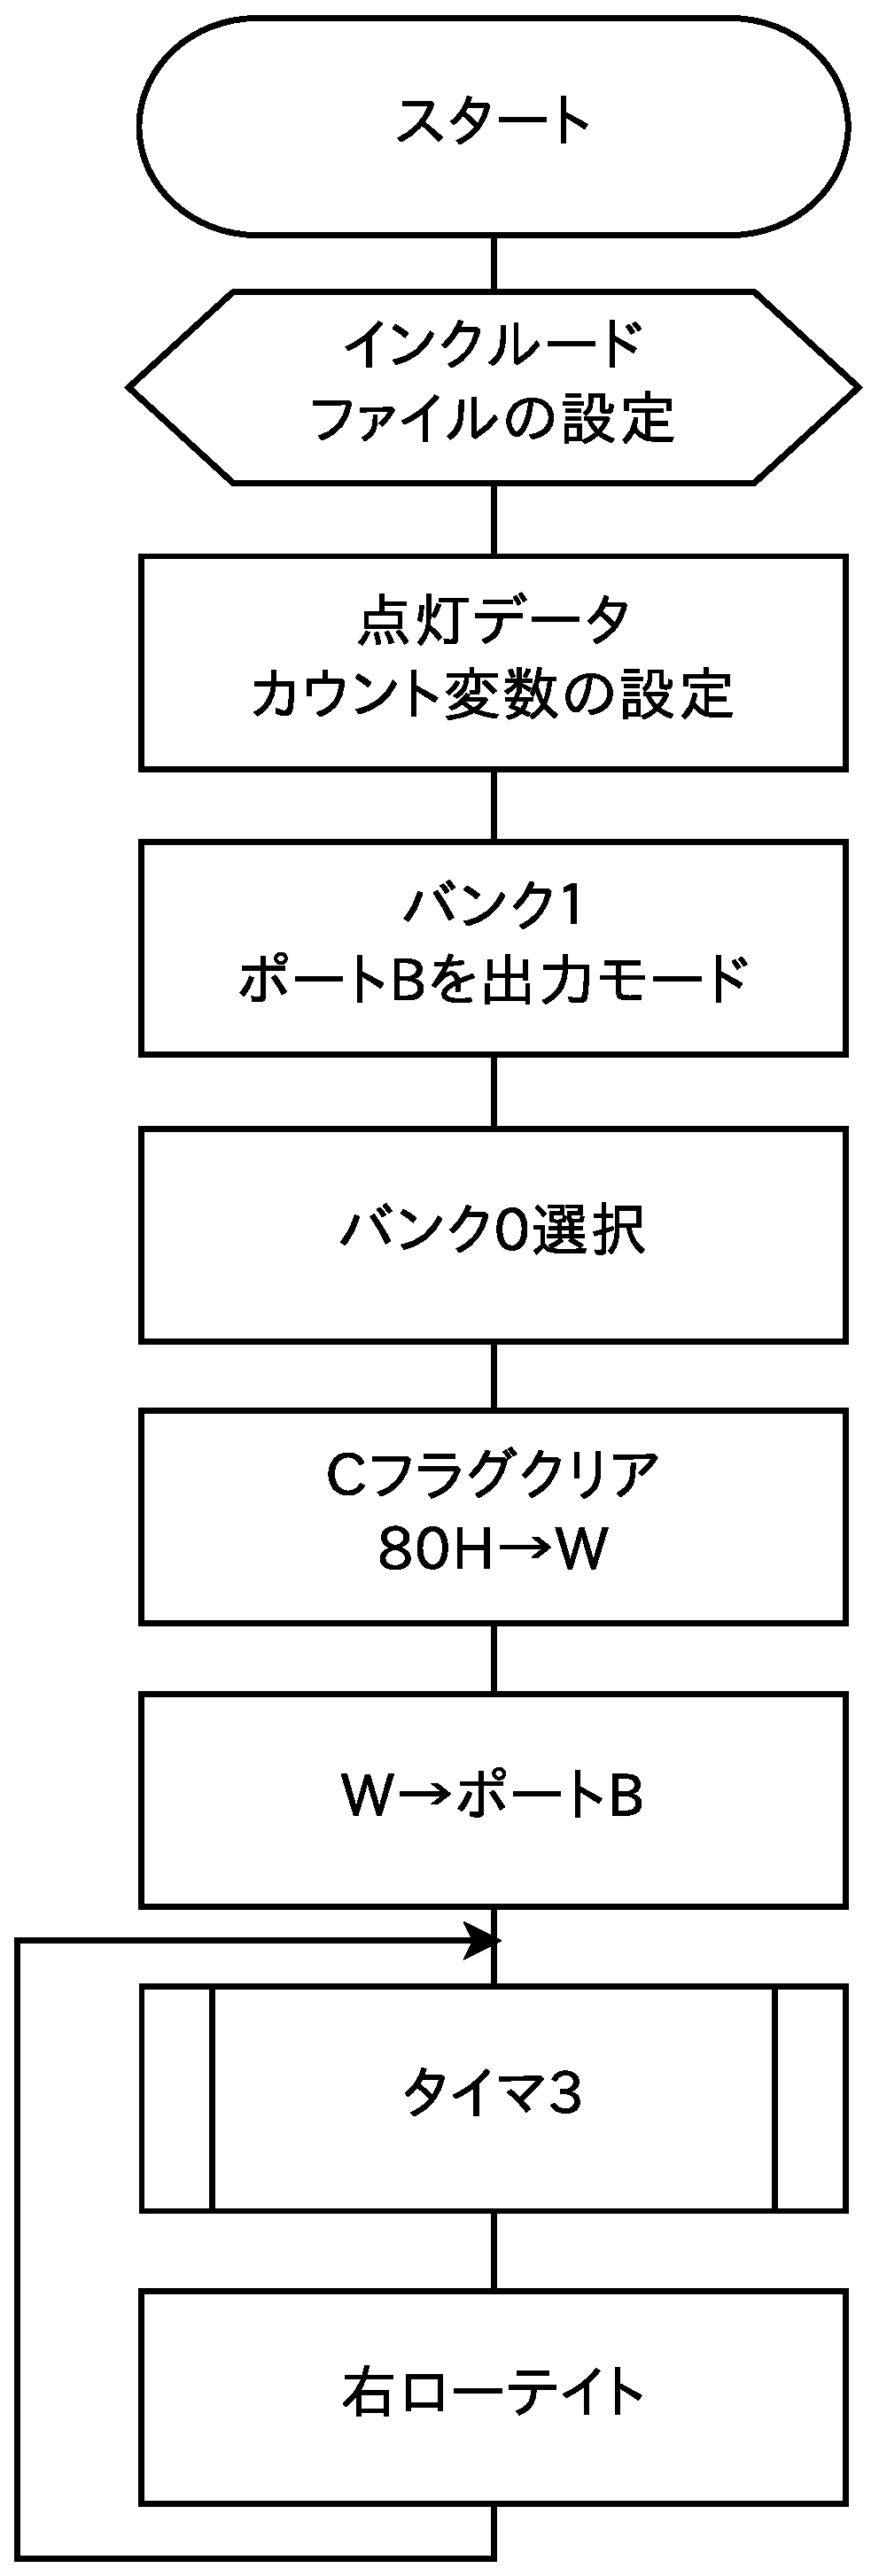
\includegraphics[height=145mm]{Diagram5-5.eps}
    \end{center}
   \caption{フローチャート}
   \label{fig}
  \end{figure}
  \subsection{ソースコード}
  \begin{lstinputlisting}[basicstyle=\ttfamily\footnotesize, frame=single]
   {../5-5/5-5.asm}
  \end{lstinputlisting}
  \subsection{実行結果}
  \begin{eqnarray*}
   {80}_{16} = 10000000_2 \\
   ●○○○○○○○ \\
   {40}_{16} = 01000000_2 \\
   ○●○○○○○○ \\
   {20}_{16} = 00100000_2 \\
   ○○●○○○○○ \\
   {10}_{16} = 00010000_2 \\
   ○○○●○○○○ \\
   {8}_{16}  = 00001000_2 \\
   ○○○○●○○○ \\
   {4}_{16}  = 00000100_2 \\
   ○○○○○●○○ \\
   {2}_{16}  = 00000010_2 \\
   ○○○○○○●○ \\
   {1}_{16}  = 00000001_2 \\
   ○○○○○○○● \\
   ●:点灯○:消灯
  \end{eqnarray*}
  このように、0.5秒毎に光る場所が、右に動いていく。
  \subsection{考察}
  ローテイト(RRF)命令は1ビットずつ右にシフトさせるもの。
  16進数で1ビット右にシフトさせることは2で割ることになる。
  \subsection{練習問題5.6}
  \begin{lstlisting}[basicstyle=\ttfamily\footnotesize, frame=single]
;       RRF     PORTB,1     ;右方向
        RLF     PORTB,1     ;左方向
  \end{lstlisting}
  このようにRRFをRLFに変更する。
  16進数で1ビット左にシフトさせることは2をかけることになる。
  \subsection{練習問題5.7}
  \begin{lstlisting}[basicstyle=\ttfamily\footnotesize, frame=single]
TIMER1  MOVLW   D'62'       ;0.1ms
        MOVWF   CNT1
LOOP1   NOP
        DECFSZ  CNT1,F
        GOTO    LOOP1
        RETURN

TIMER2  MOVLW   D'100'      ;10ms
        MOVLW   CNT2
LOOP2   NOP
        CALL    TIMER1
        DECFSZ  CNT2,F
        GOTO    LOOP2
        RETURN

TIMER3  MOVLW   D'10'       ;0.1s
        MOVWF   CNT3
LOOP3   NOP
        CALL    TIMER2
        DECFSZ  CNT3,F
        GOTO    LOOP3
        RETURN
  \end{lstlisting}
  このようにタイマのところを変更する。
  \clearpage
 \section{リスト5-6(光が流れるプログラム(往復バージョン))}
  \subsection{フローチャート}
  \begin{figure}[htbp]
   \begin{center}
    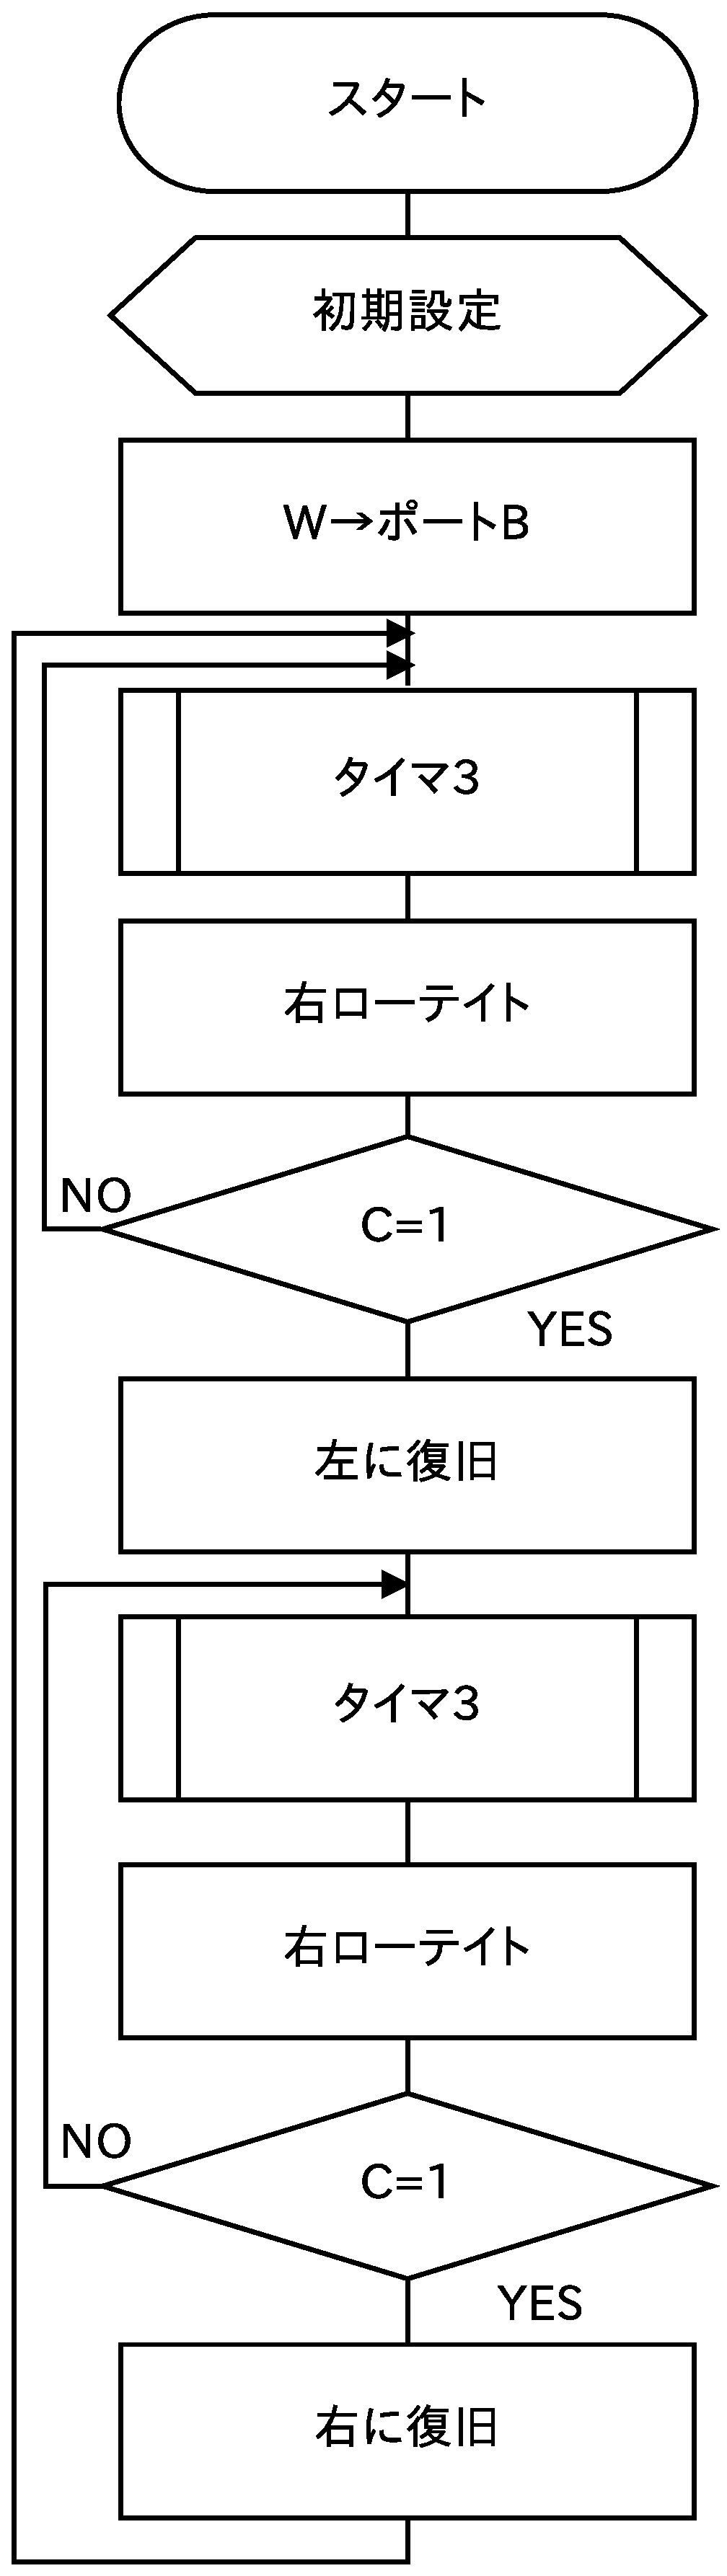
\includegraphics[height=145mm]{Diagram5-6.eps}
   \end{center}
   \caption{フローチャート}
   \label{fig}
  \end{figure}
  \subsection{ソースコード}
  \begin{lstinputlisting}[basicstyle=\ttfamily\footnotesize, frame=single]
   {../5-6/5-6.asm}
  \end{lstinputlisting}
  \subsection{実行結果}
  \begin{eqnarray*}
   {80}_{16} = 10000000_2 \\
   ●○○○○○○○ \\
   {40}_{16} = 01000000_2 \\
   ○●○○○○○○ \\
   {20}_{16} = 00100000_2 \\
   ○○●○○○○○ \\
   {10}_{16} = 00010000_2 \\
   ○○○●○○○○ \\
   {8}_{16}  = 00001000_2 \\
   ○○○○●○○○ \\
   {4}_{16}  = 00000100_2 \\
   ○○○○○●○○ \\
   {2}_{16}  = 00000010_2 \\
   ○○○○○○●○ \\
   {1}_{16}  = 00000001_2 \\
   ○○○○○○○● \\
   {2}_{16}  = 00000010_2 \\
   ○○○○○○●○ \\
   {4}_{16}  = 00000100_2 \\
   ○○○○○●○○ \\
   {8}_{16}  = 00001000_2 \\
   ○○○○●○○○ \\
   {10}_{16} = 00010000_2 \\
   ○○○●○○○○ \\
   {20}_{16} = 00100000_2 \\
   ○○●○○○○○ \\
   {40}_{16} = 01000000_2 \\
   ○●○○○○○○ \\
   {80}_{16} = 10000000_2 \\
   ●○○○○○○○ \\
   ●:点灯○:消灯
  \end{eqnarray*}
  0.2秒毎に光るところが右に動いていき右端になったら、左方向に戻ってくる。
  \subsection{考察}
  ローテイト命令は、Cフラグを含めてシフトするので、光が右端(0ビット目)または左端(7ビット目)に移動したことをCフラグで判定。
  Cフラグが1の場合はオーバーフローかアンダーフローしているので、過分ローテイトの復旧(2ビット復旧)することで、なめらかに移動するように見える。
  \subsection{練習問題5.8}
  \begin{lstlisting}[basicstyle=\ttfamily\footnotesize, frame=single]
LEDD     EQU     80H    ;左端から右方向にスタート
;LEDD    EQU     01H    ;右端から左方向にスタート
  \end{lstlisting}
  このように、LEDDのデータを80Hから01Hに変更する。
  \subsection{練習問題5.9}
  過分ローテイトの復旧がないと、すべてのLEDが点灯しない瞬間が生じる。
  \subsection{練習問題5.10}
  \clearpage
 \section{リスト5-7(スイッチ入力プログラム)}
  \subsection{フローチャート}
  \begin{figure}[htbp]
   \begin{center}
    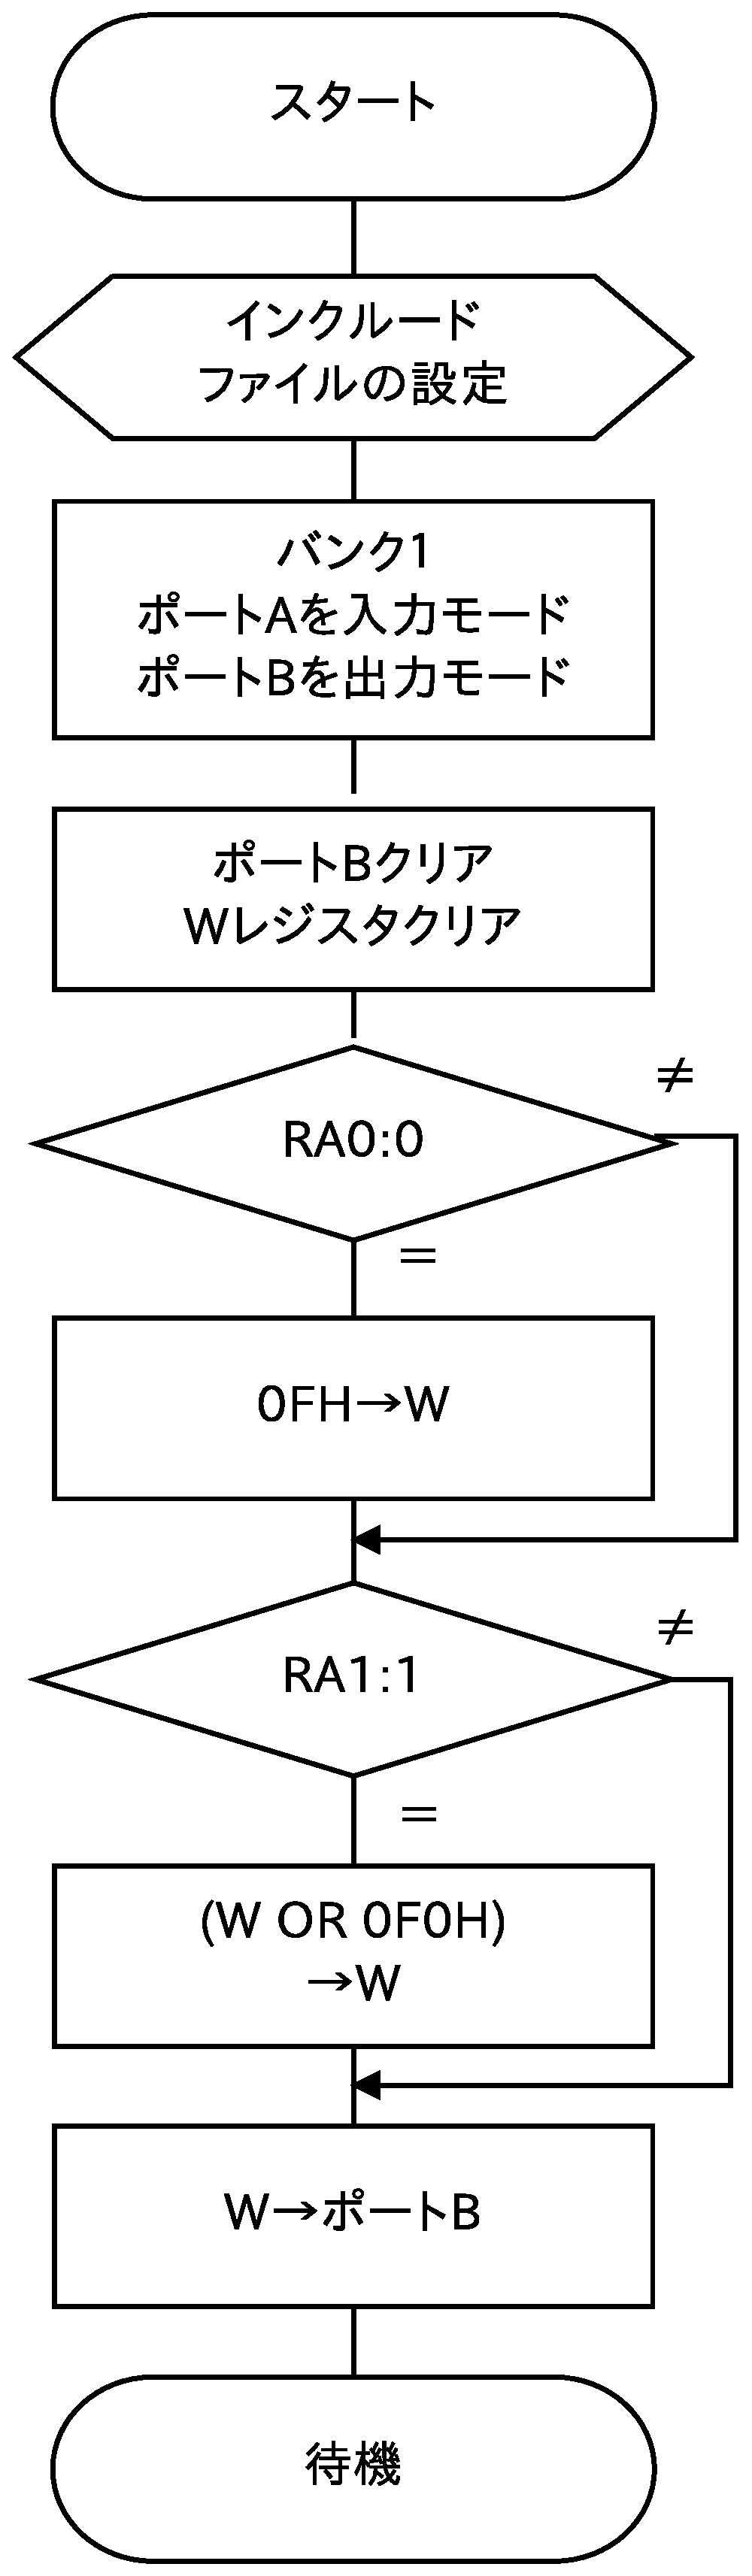
\includegraphics[height=145mm]{Diagram5-7.eps}
   \end{center}
   \caption{フローチャート}
   \label{fig}
  \end{figure}
  \clearpage
  \subsection{ソースコード}
  \begin{lstinputlisting}[basicstyle=\ttfamily\footnotesize, frame=single]
   {../5-7/5-7.asm}
  \end{lstinputlisting}
  \subsection{実行結果}
  \subsection{考察}
 \section{リスト5-8(リレー制御プログラム)}
  \subsection{フローチャート}
  \begin{figure}[htbp]
   \begin{center}
    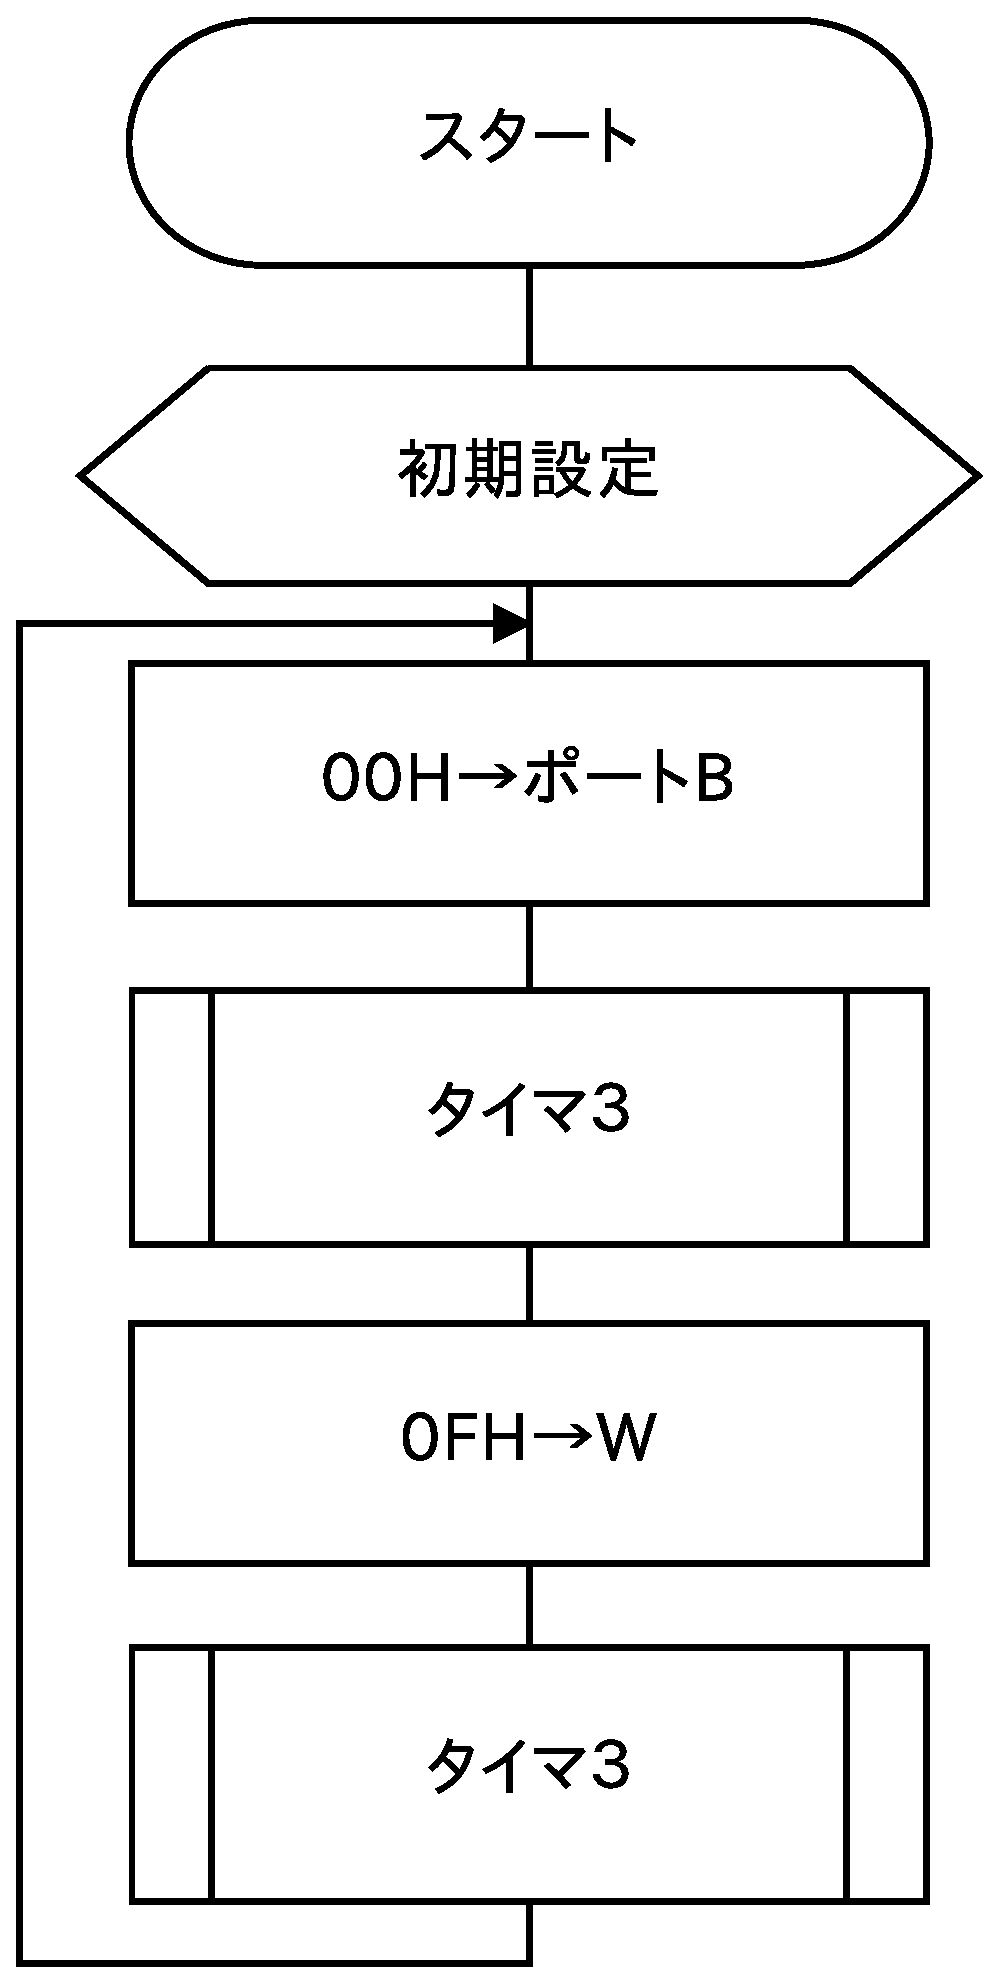
\includegraphics[height=145mm]{Diagram5-8.eps}
   \end{center}
   \caption{フローチャート}
   \label{fig}
  \end{figure}
  \clearpage
  \subsection{ソースコード}
  \begin{lstinputlisting}[basicstyle=\ttfamily\footnotesize, frame=single]
   {../5-8/5-8.asm}
  \end{lstinputlisting}
  \subsection{実行結果}
  \subsection{考察}
\end{document}